\batchmode
\documentclass[twoside]{book}

% Packages required by doxygen
\usepackage{fixltx2e}
\usepackage{calc}
\usepackage{doxygen}
\usepackage[export]{adjustbox} % also loads graphicx
\usepackage{graphicx}
\usepackage[utf8]{inputenc}
\usepackage{makeidx}
\usepackage{multicol}
\usepackage{multirow}
\PassOptionsToPackage{warn}{textcomp}
\usepackage{textcomp}
\usepackage[nointegrals]{wasysym}
\usepackage[table]{xcolor}

% Font selection
\usepackage[T1]{fontenc}
\usepackage[scaled=.90]{helvet}
\usepackage{courier}
\usepackage{amssymb}
\usepackage{sectsty}
\renewcommand{\familydefault}{\sfdefault}
\allsectionsfont{%
  \fontseries{bc}\selectfont%
  \color{darkgray}%
}
\renewcommand{\DoxyLabelFont}{%
  \fontseries{bc}\selectfont%
  \color{darkgray}%
}
\newcommand{\+}{\discretionary{\mbox{\scriptsize$\hookleftarrow$}}{}{}}

% Page & text layout
\usepackage{geometry}
\geometry{%
  a4paper,%
  top=2.5cm,%
  bottom=2.5cm,%
  left=2.5cm,%
  right=2.5cm%
}
\tolerance=750
\hfuzz=15pt
\hbadness=750
\setlength{\emergencystretch}{15pt}
\setlength{\parindent}{0cm}
\setlength{\parskip}{3ex plus 2ex minus 2ex}
\makeatletter
\renewcommand{\paragraph}{%
  \@startsection{paragraph}{4}{0ex}{-1.0ex}{1.0ex}{%
    \normalfont\normalsize\bfseries\SS@parafont%
  }%
}
\renewcommand{\subparagraph}{%
  \@startsection{subparagraph}{5}{0ex}{-1.0ex}{1.0ex}{%
    \normalfont\normalsize\bfseries\SS@subparafont%
  }%
}
\makeatother

% Headers & footers
\usepackage{fancyhdr}
\pagestyle{fancyplain}
\fancyhead[LE]{\fancyplain{}{\bfseries\thepage}}
\fancyhead[CE]{\fancyplain{}{}}
\fancyhead[RE]{\fancyplain{}{\bfseries\leftmark}}
\fancyhead[LO]{\fancyplain{}{\bfseries\rightmark}}
\fancyhead[CO]{\fancyplain{}{}}
\fancyhead[RO]{\fancyplain{}{\bfseries\thepage}}
\fancyfoot[LE]{\fancyplain{}{}}
\fancyfoot[CE]{\fancyplain{}{}}
\fancyfoot[RE]{\fancyplain{}{\bfseries\scriptsize Generated by Doxygen }}
\fancyfoot[LO]{\fancyplain{}{\bfseries\scriptsize Generated by Doxygen }}
\fancyfoot[CO]{\fancyplain{}{}}
\fancyfoot[RO]{\fancyplain{}{}}
\renewcommand{\footrulewidth}{0.4pt}
\renewcommand{\chaptermark}[1]{%
  \markboth{#1}{}%
}
\renewcommand{\sectionmark}[1]{%
  \markright{\thesection\ #1}%
}

% Indices & bibliography
\usepackage{natbib}
\usepackage[titles]{tocloft}
\setcounter{tocdepth}{3}
\setcounter{secnumdepth}{5}
\makeindex

% Hyperlinks (required, but should be loaded last)
\usepackage{ifpdf}
\ifpdf
  \usepackage[pdftex,pagebackref=true]{hyperref}
\else
  \usepackage[ps2pdf,pagebackref=true]{hyperref}
\fi
\hypersetup{%
  colorlinks=true,%
  linkcolor=blue,%
  citecolor=blue,%
  unicode%
}

% Custom commands
\newcommand{\clearemptydoublepage}{%
  \newpage{\pagestyle{empty}\cleardoublepage}%
}

\usepackage{caption}
\captionsetup{labelsep=space,justification=centering,font={bf},singlelinecheck=off,skip=4pt,position=top}

%===== C O N T E N T S =====

\begin{document}

% Titlepage & ToC
\hypersetup{pageanchor=false,
             bookmarksnumbered=true
            }
\pagenumbering{alph}
\pagenumbering{arabic}
\hypersetup{pageanchor=true}

%--- Begin generated contents ---
\chapter{Example problem\+: 2D driven cavity flow in a quarter-\/circle domain with spatial adaptation.}
\label{index}\hypertarget{index}{}\hypertarget{index_q}{}\section{A few quick questions...}\label{index_q}
Since {\ttfamily oomph-\/lib} is developed as open-\/source software, any evidence that the code is being downloaded and used is very helpful for us as it helps to justify our continued work on this project.

We would therefore be extremely grateful if you could provide the information requested in the form below. Pressing the \char`\"{}submit\char`\"{} button will get you to the actual download page.

{\bfseries Note\+:} 
\begin{DoxyItemize}
\item All information will be treated as confidential. 
\item If you provide your email address and check the appropriate box we will add you to our mailing list to inform you of upgrades and bug fixes to the code. Rest assured that the mailing list is {\bfseries very low volume} -- we have better things to do than to bombard you with email. 
\item If you still feel reluctant to provide any of the information requested, feel free to enter some dummy input. The form will check that {\bfseries some} information has been entered but entering your name as \char`\"{}\+Joe Cool\char`\"{} is perfectly acceptable -- this is to discourage people from not providing the information simply because they are too lazy to type... 
\end{DoxyItemize}



 







 

 \hypertarget{index_pdf}{}\section{P\+D\+F file}\label{index_pdf}
A \href{../latex/refman.pdf}{\tt pdf version} of this document is available. \end{document}

\chapter{Namespace Index}
\section{Namespace List}
Here is a list of all namespaces with brief descriptions\+:\begin{DoxyCompactList}
\item\contentsline{section}{\hyperlink{namespaceGlobal__Physical__Variables}{Global\+\_\+\+Physical\+\_\+\+Variables} \\*Global variables that represent physical properties }{\pageref{namespaceGlobal__Physical__Variables}}{}
\item\contentsline{section}{\hyperlink{namespaceoomph}{oomph} }{\pageref{namespaceoomph}}{}
\item\contentsline{section}{\hyperlink{namespacePhysical__Variables}{Physical\+\_\+\+Variables} \\*Namespace for the solution of 2D linear shell equation }{\pageref{namespacePhysical__Variables}}{}
\end{DoxyCompactList}

\chapter{Hierarchical Index}
\section{Class Hierarchy}
This inheritance list is sorted roughly, but not completely, alphabetically\+:\begin{DoxyCompactList}
\item Problem\begin{DoxyCompactList}
\item \contentsline{section}{Unstructured\+Solid\+Problem$<$ E\+L\+E\+M\+E\+NT $>$}{\pageref{classUnstructuredSolidProblem}}{}
\end{DoxyCompactList}
\end{DoxyCompactList}

\chapter{Class Index}
\section{Class List}
Here are the classes, structs, unions and interfaces with brief descriptions\+:\begin{DoxyCompactList}
\item\contentsline{section}{\hyperlink{classPMLProblem}{P\+M\+L\+Problem$<$ E\+L\+E\+M\+E\+N\+T $>$} }{\pageref{classPMLProblem}}{}
\item\contentsline{section}{\hyperlink{classGlobalParameters_1_1TestPMLMapping}{Global\+Parameters\+::\+Test\+P\+M\+L\+Mapping} }{\pageref{classGlobalParameters_1_1TestPMLMapping}}{}
\end{DoxyCompactList}

\chapter{File Index}
\section{File List}
Here is a list of all files with brief descriptions\+:\begin{DoxyCompactList}
\item\contentsline{section}{\hyperlink{jeffery__orbit_8cc}{jeffery\+\_\+orbit.\+cc} }{\pageref{jeffery__orbit_8cc}}{}
\item\contentsline{section}{\hyperlink{jeffery__orbit_8txt__doxygenified_8h}{jeffery\+\_\+orbit.\+txt\+\_\+doxygenified.\+h} }{\pageref{jeffery__orbit_8txt__doxygenified_8h}}{}
\item\contentsline{section}{\hyperlink{my__taylor__hood__elements_8h}{my\+\_\+taylor\+\_\+hood\+\_\+elements.\+h} }{\pageref{my__taylor__hood__elements_8h}}{}
\end{DoxyCompactList}

\chapter{Namespace Documentation}
\hypertarget{namespaceGlobal__Physical__Variables}{}\section{Global\+\_\+\+Physical\+\_\+\+Variables Namespace Reference}
\label{namespaceGlobal__Physical__Variables}\index{Global\+\_\+\+Physical\+\_\+\+Variables@{Global\+\_\+\+Physical\+\_\+\+Variables}}


Namespace for physical parameters.  


\subsection*{Functions}
\begin{DoxyCompactItemize}
\item 
Vector$<$ double $>$ \hyperlink{namespaceGlobal__Physical__Variables_afae321364975eb56688ad13abc8ed6b7}{Gravity} (2)
\begin{DoxyCompactList}\small\item\em Gravity vector. \end{DoxyCompactList}\item 
void \hyperlink{namespaceGlobal__Physical__Variables_a87da705b8a46bed337cf5dbdd788b87b}{body\+\_\+force} (const double \&time, const Vector$<$ double $>$ \&x, Vector$<$ double $>$ \&result)
\begin{DoxyCompactList}\small\item\em Functional body force. \end{DoxyCompactList}\item 
void \hyperlink{namespaceGlobal__Physical__Variables_a9780d615ae07c4e00a436ab2973b54e6}{zero\+\_\+body\+\_\+force} (const double \&time, const Vector$<$ double $>$ \&x, Vector$<$ double $>$ \&result)
\begin{DoxyCompactList}\small\item\em Zero functional body force. \end{DoxyCompactList}\end{DoxyCompactItemize}
\subsection*{Variables}
\begin{DoxyCompactItemize}
\item 
double \hyperlink{namespaceGlobal__Physical__Variables_ab814e627d2eb5bc50318879d19ab16b9}{Re} =100
\begin{DoxyCompactList}\small\item\em Reynolds number. \end{DoxyCompactList}\item 
double \hyperlink{namespaceGlobal__Physical__Variables_ab1a845a672b4d74b304639a976dc65c6}{Re\+\_\+inv\+Fr} =100
\begin{DoxyCompactList}\small\item\em Reynolds/\+Froude number. \end{DoxyCompactList}\end{DoxyCompactItemize}


\subsection{Detailed Description}
Namespace for physical parameters. 

\subsection{Function Documentation}
\mbox{\Hypertarget{namespaceGlobal__Physical__Variables_a87da705b8a46bed337cf5dbdd788b87b}\label{namespaceGlobal__Physical__Variables_a87da705b8a46bed337cf5dbdd788b87b}} 
\index{Global\+\_\+\+Physical\+\_\+\+Variables@{Global\+\_\+\+Physical\+\_\+\+Variables}!body\+\_\+force@{body\+\_\+force}}
\index{body\+\_\+force@{body\+\_\+force}!Global\+\_\+\+Physical\+\_\+\+Variables@{Global\+\_\+\+Physical\+\_\+\+Variables}}
\subsubsection{\texorpdfstring{body\+\_\+force()}{body\_force()}}
{\footnotesize\ttfamily void Global\+\_\+\+Physical\+\_\+\+Variables\+::body\+\_\+force (\begin{DoxyParamCaption}\item[{const double \&}]{time,  }\item[{const Vector$<$ double $>$ \&}]{x,  }\item[{Vector$<$ double $>$ \&}]{result }\end{DoxyParamCaption})}



Functional body force. 



Definition at line 62 of file circular\+\_\+driven\+\_\+cavity.\+cc.



References Re\+\_\+inv\+Fr.



Referenced by main().

\mbox{\Hypertarget{namespaceGlobal__Physical__Variables_afae321364975eb56688ad13abc8ed6b7}\label{namespaceGlobal__Physical__Variables_afae321364975eb56688ad13abc8ed6b7}} 
\index{Global\+\_\+\+Physical\+\_\+\+Variables@{Global\+\_\+\+Physical\+\_\+\+Variables}!Gravity@{Gravity}}
\index{Gravity@{Gravity}!Global\+\_\+\+Physical\+\_\+\+Variables@{Global\+\_\+\+Physical\+\_\+\+Variables}}
\subsubsection{\texorpdfstring{Gravity()}{Gravity()}}
{\footnotesize\ttfamily Vector$<$double$>$ Global\+\_\+\+Physical\+\_\+\+Variables\+::\+Gravity (\begin{DoxyParamCaption}\item[{2}]{ }\end{DoxyParamCaption})}



Gravity vector. 



Referenced by main(), and Quarter\+Circle\+Driven\+Cavity\+Problem$<$ E\+L\+E\+M\+E\+N\+T $>$\+::\+Quarter\+Circle\+Driven\+Cavity\+Problem().

\mbox{\Hypertarget{namespaceGlobal__Physical__Variables_a9780d615ae07c4e00a436ab2973b54e6}\label{namespaceGlobal__Physical__Variables_a9780d615ae07c4e00a436ab2973b54e6}} 
\index{Global\+\_\+\+Physical\+\_\+\+Variables@{Global\+\_\+\+Physical\+\_\+\+Variables}!zero\+\_\+body\+\_\+force@{zero\+\_\+body\+\_\+force}}
\index{zero\+\_\+body\+\_\+force@{zero\+\_\+body\+\_\+force}!Global\+\_\+\+Physical\+\_\+\+Variables@{Global\+\_\+\+Physical\+\_\+\+Variables}}
\subsubsection{\texorpdfstring{zero\+\_\+body\+\_\+force()}{zero\_body\_force()}}
{\footnotesize\ttfamily void Global\+\_\+\+Physical\+\_\+\+Variables\+::zero\+\_\+body\+\_\+force (\begin{DoxyParamCaption}\item[{const double \&}]{time,  }\item[{const Vector$<$ double $>$ \&}]{x,  }\item[{Vector$<$ double $>$ \&}]{result }\end{DoxyParamCaption})}



Zero functional body force. 



Definition at line 70 of file circular\+\_\+driven\+\_\+cavity.\+cc.



Referenced by main().



\subsection{Variable Documentation}
\mbox{\Hypertarget{namespaceGlobal__Physical__Variables_ab814e627d2eb5bc50318879d19ab16b9}\label{namespaceGlobal__Physical__Variables_ab814e627d2eb5bc50318879d19ab16b9}} 
\index{Global\+\_\+\+Physical\+\_\+\+Variables@{Global\+\_\+\+Physical\+\_\+\+Variables}!Re@{Re}}
\index{Re@{Re}!Global\+\_\+\+Physical\+\_\+\+Variables@{Global\+\_\+\+Physical\+\_\+\+Variables}}
\subsubsection{\texorpdfstring{Re}{Re}}
{\footnotesize\ttfamily double Global\+\_\+\+Physical\+\_\+\+Variables\+::\+Re =100}



Reynolds number. 



Definition at line 53 of file circular\+\_\+driven\+\_\+cavity.\+cc.



Referenced by Quarter\+Circle\+Driven\+Cavity\+Problem$<$ E\+L\+E\+M\+E\+N\+T $>$\+::\+Quarter\+Circle\+Driven\+Cavity\+Problem().

\mbox{\Hypertarget{namespaceGlobal__Physical__Variables_ab1a845a672b4d74b304639a976dc65c6}\label{namespaceGlobal__Physical__Variables_ab1a845a672b4d74b304639a976dc65c6}} 
\index{Global\+\_\+\+Physical\+\_\+\+Variables@{Global\+\_\+\+Physical\+\_\+\+Variables}!Re\+\_\+inv\+Fr@{Re\+\_\+inv\+Fr}}
\index{Re\+\_\+inv\+Fr@{Re\+\_\+inv\+Fr}!Global\+\_\+\+Physical\+\_\+\+Variables@{Global\+\_\+\+Physical\+\_\+\+Variables}}
\subsubsection{\texorpdfstring{Re\+\_\+inv\+Fr}{Re\_invFr}}
{\footnotesize\ttfamily double Global\+\_\+\+Physical\+\_\+\+Variables\+::\+Re\+\_\+inv\+Fr =100}



Reynolds/\+Froude number. 



Definition at line 56 of file circular\+\_\+driven\+\_\+cavity.\+cc.



Referenced by body\+\_\+force(), and Quarter\+Circle\+Driven\+Cavity\+Problem$<$ E\+L\+E\+M\+E\+N\+T $>$\+::\+Quarter\+Circle\+Driven\+Cavity\+Problem().


\hypertarget{namespaceGlobal__Physical__Variables2}{}\section{Global\+\_\+\+Physical\+\_\+\+Variables2 Namespace Reference}
\label{namespaceGlobal__Physical__Variables2}\index{Global\+\_\+\+Physical\+\_\+\+Variables2@{Global\+\_\+\+Physical\+\_\+\+Variables2}}


Namespace for physical parameters.  


\subsection*{Variables}
\begin{DoxyCompactItemize}
\item 
double \hyperlink{namespaceGlobal__Physical__Variables2_afce617c1bd6726b29fa0e1f7c892a955}{Re} =100
\begin{DoxyCompactList}\small\item\em Reynolds number. \end{DoxyCompactList}\end{DoxyCompactItemize}


\subsection{Detailed Description}
Namespace for physical parameters. 

\subsection{Variable Documentation}
\mbox{\Hypertarget{namespaceGlobal__Physical__Variables2_afce617c1bd6726b29fa0e1f7c892a955}\label{namespaceGlobal__Physical__Variables2_afce617c1bd6726b29fa0e1f7c892a955}} 
\index{Global\+\_\+\+Physical\+\_\+\+Variables2@{Global\+\_\+\+Physical\+\_\+\+Variables2}!Re@{Re}}
\index{Re@{Re}!Global\+\_\+\+Physical\+\_\+\+Variables2@{Global\+\_\+\+Physical\+\_\+\+Variables2}}
\subsubsection{\texorpdfstring{Re}{Re}}
{\footnotesize\ttfamily double Global\+\_\+\+Physical\+\_\+\+Variables2\+::\+Re =100}



Reynolds number. 



Definition at line 52 of file spine\+\_\+channel2.\+cc.



Referenced by Spiked\+Channel\+Spine\+Flow\+Problem$<$ E\+L\+E\+M\+E\+N\+T $>$\+::\+Spiked\+Channel\+Spine\+Flow\+Problem().


\chapter{Class Documentation}
\hypertarget{classQuarterCircleDrivenCavityProblem}{}\section{Quarter\+Circle\+Driven\+Cavity\+Problem$<$ E\+L\+E\+M\+E\+NT $>$ Class Template Reference}
\label{classQuarterCircleDrivenCavityProblem}\index{Quarter\+Circle\+Driven\+Cavity\+Problem$<$ E\+L\+E\+M\+E\+N\+T $>$@{Quarter\+Circle\+Driven\+Cavity\+Problem$<$ E\+L\+E\+M\+E\+N\+T $>$}}
Inheritance diagram for Quarter\+Circle\+Driven\+Cavity\+Problem$<$ E\+L\+E\+M\+E\+NT $>$\+:\begin{figure}[H]
\begin{center}
\leavevmode
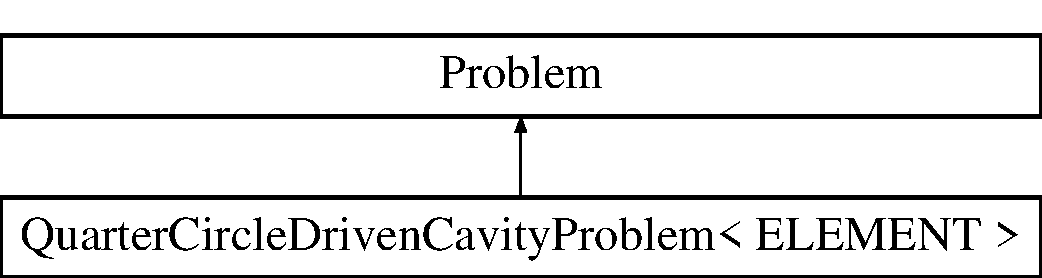
\includegraphics[height=2.000000cm]{classQuarterCircleDrivenCavityProblem}
\end{center}
\end{figure}
\subsection*{Public Member Functions}
\begin{DoxyCompactItemize}
\item 
\hyperlink{classQuarterCircleDrivenCavityProblem_ae5fd69acf7d28a600cb6aa0bbb6a341c}{Quarter\+Circle\+Driven\+Cavity\+Problem} (Navier\+Stokes\+Equations$<$ 2 $>$\+::Navier\+Stokes\+Body\+Force\+Fct\+Pt body\+\_\+force\+\_\+fct\+\_\+pt)
\begin{DoxyCompactList}\small\item\em Constructor. \end{DoxyCompactList}\item 
\hyperlink{classQuarterCircleDrivenCavityProblem_a07410fd9d1194613f92dd6620fa3207a}{$\sim$\+Quarter\+Circle\+Driven\+Cavity\+Problem} ()
\begin{DoxyCompactList}\small\item\em Destructor\+: Empty. \end{DoxyCompactList}\item 
void \hyperlink{classQuarterCircleDrivenCavityProblem_ad2ed0b3e89e1cd0e28cc61ae4fd129bc}{actions\+\_\+after\+\_\+newton\+\_\+solve} ()
\begin{DoxyCompactList}\small\item\em Update the after solve (empty) \end{DoxyCompactList}\item 
void \hyperlink{classQuarterCircleDrivenCavityProblem_aa1d9cfd27fc1abe2a85e756009781547}{actions\+\_\+before\+\_\+newton\+\_\+solve} ()
\begin{DoxyCompactList}\small\item\em Update the problem specs before solve. (Re-\/)set velocity boundary conditions just to be on the safe side... \end{DoxyCompactList}\item 
void \hyperlink{classQuarterCircleDrivenCavityProblem_a4873f31ccf76e340abb284b17430c407}{actions\+\_\+after\+\_\+adapt} ()
\begin{DoxyCompactList}\small\item\em After adaptation\+: Unpin pressure and pin redudant pressure dofs. \end{DoxyCompactList}\item 
void \hyperlink{classQuarterCircleDrivenCavityProblem_a390b7b3c027a0253a2a3ac42f9715736}{doc\+\_\+solution} (Doc\+Info \&doc\+\_\+info)
\begin{DoxyCompactList}\small\item\em Doc the solution. \end{DoxyCompactList}\end{DoxyCompactItemize}
\subsection*{Private Member Functions}
\begin{DoxyCompactItemize}
\item 
void \hyperlink{classQuarterCircleDrivenCavityProblem_a0c4e0cb1a4fb12053142fa43f899a5b1}{fix\+\_\+pressure} (const unsigned \&e, const unsigned \&pdof, const double \&pvalue)
\begin{DoxyCompactList}\small\item\em Fix pressure in element e at pressure dof pdof and set to pvalue. \end{DoxyCompactList}\end{DoxyCompactItemize}
\subsection*{Private Attributes}
\begin{DoxyCompactItemize}
\item 
Navier\+Stokes\+Equations$<$ 2 $>$\+::Navier\+Stokes\+Body\+Force\+Fct\+Pt \hyperlink{classQuarterCircleDrivenCavityProblem_a66bd39fdcb467ebdb6afe9446d4566f3}{Body\+\_\+force\+\_\+fct\+\_\+pt}
\begin{DoxyCompactList}\small\item\em Pointer to body force function. \end{DoxyCompactList}\end{DoxyCompactItemize}


\subsection{Detailed Description}
\subsubsection*{template$<$class E\+L\+E\+M\+E\+NT$>$\newline
class Quarter\+Circle\+Driven\+Cavity\+Problem$<$ E\+L\+E\+M\+E\+N\+T $>$}

Driven cavity problem in quarter circle domain, templated by element type. 

Definition at line 88 of file circular\+\_\+driven\+\_\+cavity.\+cc.



\subsection{Constructor \& Destructor Documentation}
\mbox{\Hypertarget{classQuarterCircleDrivenCavityProblem_ae5fd69acf7d28a600cb6aa0bbb6a341c}\label{classQuarterCircleDrivenCavityProblem_ae5fd69acf7d28a600cb6aa0bbb6a341c}} 
\index{Quarter\+Circle\+Driven\+Cavity\+Problem@{Quarter\+Circle\+Driven\+Cavity\+Problem}!Quarter\+Circle\+Driven\+Cavity\+Problem@{Quarter\+Circle\+Driven\+Cavity\+Problem}}
\index{Quarter\+Circle\+Driven\+Cavity\+Problem@{Quarter\+Circle\+Driven\+Cavity\+Problem}!Quarter\+Circle\+Driven\+Cavity\+Problem@{Quarter\+Circle\+Driven\+Cavity\+Problem}}
\subsubsection{\texorpdfstring{Quarter\+Circle\+Driven\+Cavity\+Problem()}{QuarterCircleDrivenCavityProblem()}}
{\footnotesize\ttfamily template$<$class E\+L\+E\+M\+E\+NT $>$ \\
\hyperlink{classQuarterCircleDrivenCavityProblem}{Quarter\+Circle\+Driven\+Cavity\+Problem}$<$ E\+L\+E\+M\+E\+NT $>$\+::\hyperlink{classQuarterCircleDrivenCavityProblem}{Quarter\+Circle\+Driven\+Cavity\+Problem} (\begin{DoxyParamCaption}\item[{Navier\+Stokes\+Equations$<$ 2 $>$\+::Navier\+Stokes\+Body\+Force\+Fct\+Pt}]{body\+\_\+force\+\_\+fct\+\_\+pt }\end{DoxyParamCaption})}



Constructor. 

Constructor for driven cavity problem in quarter circle domain. 

Definition at line 176 of file circular\+\_\+driven\+\_\+cavity.\+cc.



References Quarter\+Circle\+Driven\+Cavity\+Problem$<$ E\+L\+E\+M\+E\+N\+T $>$\+::\+Body\+\_\+force\+\_\+fct\+\_\+pt, Quarter\+Circle\+Driven\+Cavity\+Problem$<$ E\+L\+E\+M\+E\+N\+T $>$\+::fix\+\_\+pressure(), Global\+\_\+\+Physical\+\_\+\+Variables\+::\+Gravity(), Global\+\_\+\+Physical\+\_\+\+Variables\+::\+Re, and Global\+\_\+\+Physical\+\_\+\+Variables\+::\+Re\+\_\+inv\+Fr.

\mbox{\Hypertarget{classQuarterCircleDrivenCavityProblem_a07410fd9d1194613f92dd6620fa3207a}\label{classQuarterCircleDrivenCavityProblem_a07410fd9d1194613f92dd6620fa3207a}} 
\index{Quarter\+Circle\+Driven\+Cavity\+Problem@{Quarter\+Circle\+Driven\+Cavity\+Problem}!````~Quarter\+Circle\+Driven\+Cavity\+Problem@{$\sim$\+Quarter\+Circle\+Driven\+Cavity\+Problem}}
\index{````~Quarter\+Circle\+Driven\+Cavity\+Problem@{$\sim$\+Quarter\+Circle\+Driven\+Cavity\+Problem}!Quarter\+Circle\+Driven\+Cavity\+Problem@{Quarter\+Circle\+Driven\+Cavity\+Problem}}
\subsubsection{\texorpdfstring{$\sim$\+Quarter\+Circle\+Driven\+Cavity\+Problem()}{~QuarterCircleDrivenCavityProblem()}}
{\footnotesize\ttfamily template$<$class E\+L\+E\+M\+E\+NT$>$ \\
\hyperlink{classQuarterCircleDrivenCavityProblem}{Quarter\+Circle\+Driven\+Cavity\+Problem}$<$ E\+L\+E\+M\+E\+NT $>$\+::$\sim$\hyperlink{classQuarterCircleDrivenCavityProblem}{Quarter\+Circle\+Driven\+Cavity\+Problem} (\begin{DoxyParamCaption}{ }\end{DoxyParamCaption})\hspace{0.3cm}{\ttfamily [inline]}}



Destructor\+: Empty. 



Definition at line 98 of file circular\+\_\+driven\+\_\+cavity.\+cc.



\subsection{Member Function Documentation}
\mbox{\Hypertarget{classQuarterCircleDrivenCavityProblem_a4873f31ccf76e340abb284b17430c407}\label{classQuarterCircleDrivenCavityProblem_a4873f31ccf76e340abb284b17430c407}} 
\index{Quarter\+Circle\+Driven\+Cavity\+Problem@{Quarter\+Circle\+Driven\+Cavity\+Problem}!actions\+\_\+after\+\_\+adapt@{actions\+\_\+after\+\_\+adapt}}
\index{actions\+\_\+after\+\_\+adapt@{actions\+\_\+after\+\_\+adapt}!Quarter\+Circle\+Driven\+Cavity\+Problem@{Quarter\+Circle\+Driven\+Cavity\+Problem}}
\subsubsection{\texorpdfstring{actions\+\_\+after\+\_\+adapt()}{actions\_after\_adapt()}}
{\footnotesize\ttfamily template$<$class E\+L\+E\+M\+E\+NT$>$ \\
void \hyperlink{classQuarterCircleDrivenCavityProblem}{Quarter\+Circle\+Driven\+Cavity\+Problem}$<$ E\+L\+E\+M\+E\+NT $>$\+::actions\+\_\+after\+\_\+adapt (\begin{DoxyParamCaption}{ }\end{DoxyParamCaption})\hspace{0.3cm}{\ttfamily [inline]}}



After adaptation\+: Unpin pressure and pin redudant pressure dofs. 



Definition at line 137 of file circular\+\_\+driven\+\_\+cavity.\+cc.

\mbox{\Hypertarget{classQuarterCircleDrivenCavityProblem_ad2ed0b3e89e1cd0e28cc61ae4fd129bc}\label{classQuarterCircleDrivenCavityProblem_ad2ed0b3e89e1cd0e28cc61ae4fd129bc}} 
\index{Quarter\+Circle\+Driven\+Cavity\+Problem@{Quarter\+Circle\+Driven\+Cavity\+Problem}!actions\+\_\+after\+\_\+newton\+\_\+solve@{actions\+\_\+after\+\_\+newton\+\_\+solve}}
\index{actions\+\_\+after\+\_\+newton\+\_\+solve@{actions\+\_\+after\+\_\+newton\+\_\+solve}!Quarter\+Circle\+Driven\+Cavity\+Problem@{Quarter\+Circle\+Driven\+Cavity\+Problem}}
\subsubsection{\texorpdfstring{actions\+\_\+after\+\_\+newton\+\_\+solve()}{actions\_after\_newton\_solve()}}
{\footnotesize\ttfamily template$<$class E\+L\+E\+M\+E\+NT$>$ \\
void \hyperlink{classQuarterCircleDrivenCavityProblem}{Quarter\+Circle\+Driven\+Cavity\+Problem}$<$ E\+L\+E\+M\+E\+NT $>$\+::actions\+\_\+after\+\_\+newton\+\_\+solve (\begin{DoxyParamCaption}{ }\end{DoxyParamCaption})\hspace{0.3cm}{\ttfamily [inline]}}



Update the after solve (empty) 



Definition at line 101 of file circular\+\_\+driven\+\_\+cavity.\+cc.

\mbox{\Hypertarget{classQuarterCircleDrivenCavityProblem_aa1d9cfd27fc1abe2a85e756009781547}\label{classQuarterCircleDrivenCavityProblem_aa1d9cfd27fc1abe2a85e756009781547}} 
\index{Quarter\+Circle\+Driven\+Cavity\+Problem@{Quarter\+Circle\+Driven\+Cavity\+Problem}!actions\+\_\+before\+\_\+newton\+\_\+solve@{actions\+\_\+before\+\_\+newton\+\_\+solve}}
\index{actions\+\_\+before\+\_\+newton\+\_\+solve@{actions\+\_\+before\+\_\+newton\+\_\+solve}!Quarter\+Circle\+Driven\+Cavity\+Problem@{Quarter\+Circle\+Driven\+Cavity\+Problem}}
\subsubsection{\texorpdfstring{actions\+\_\+before\+\_\+newton\+\_\+solve()}{actions\_before\_newton\_solve()}}
{\footnotesize\ttfamily template$<$class E\+L\+E\+M\+E\+NT$>$ \\
void \hyperlink{classQuarterCircleDrivenCavityProblem}{Quarter\+Circle\+Driven\+Cavity\+Problem}$<$ E\+L\+E\+M\+E\+NT $>$\+::actions\+\_\+before\+\_\+newton\+\_\+solve (\begin{DoxyParamCaption}{ }\end{DoxyParamCaption})\hspace{0.3cm}{\ttfamily [inline]}}



Update the problem specs before solve. (Re-\/)set velocity boundary conditions just to be on the safe side... 



Definition at line 105 of file circular\+\_\+driven\+\_\+cavity.\+cc.

\mbox{\Hypertarget{classQuarterCircleDrivenCavityProblem_a390b7b3c027a0253a2a3ac42f9715736}\label{classQuarterCircleDrivenCavityProblem_a390b7b3c027a0253a2a3ac42f9715736}} 
\index{Quarter\+Circle\+Driven\+Cavity\+Problem@{Quarter\+Circle\+Driven\+Cavity\+Problem}!doc\+\_\+solution@{doc\+\_\+solution}}
\index{doc\+\_\+solution@{doc\+\_\+solution}!Quarter\+Circle\+Driven\+Cavity\+Problem@{Quarter\+Circle\+Driven\+Cavity\+Problem}}
\subsubsection{\texorpdfstring{doc\+\_\+solution()}{doc\_solution()}}
{\footnotesize\ttfamily template$<$class E\+L\+E\+M\+E\+NT $>$ \\
void \hyperlink{classQuarterCircleDrivenCavityProblem}{Quarter\+Circle\+Driven\+Cavity\+Problem}$<$ E\+L\+E\+M\+E\+NT $>$\+::doc\+\_\+solution (\begin{DoxyParamCaption}\item[{Doc\+Info \&}]{doc\+\_\+info }\end{DoxyParamCaption})}



Doc the solution. 



Definition at line 267 of file circular\+\_\+driven\+\_\+cavity.\+cc.



Referenced by main().

\mbox{\Hypertarget{classQuarterCircleDrivenCavityProblem_a0c4e0cb1a4fb12053142fa43f899a5b1}\label{classQuarterCircleDrivenCavityProblem_a0c4e0cb1a4fb12053142fa43f899a5b1}} 
\index{Quarter\+Circle\+Driven\+Cavity\+Problem@{Quarter\+Circle\+Driven\+Cavity\+Problem}!fix\+\_\+pressure@{fix\+\_\+pressure}}
\index{fix\+\_\+pressure@{fix\+\_\+pressure}!Quarter\+Circle\+Driven\+Cavity\+Problem@{Quarter\+Circle\+Driven\+Cavity\+Problem}}
\subsubsection{\texorpdfstring{fix\+\_\+pressure()}{fix\_pressure()}}
{\footnotesize\ttfamily template$<$class E\+L\+E\+M\+E\+NT$>$ \\
void \hyperlink{classQuarterCircleDrivenCavityProblem}{Quarter\+Circle\+Driven\+Cavity\+Problem}$<$ E\+L\+E\+M\+E\+NT $>$\+::fix\+\_\+pressure (\begin{DoxyParamCaption}\item[{const unsigned \&}]{e,  }\item[{const unsigned \&}]{pdof,  }\item[{const double \&}]{pvalue }\end{DoxyParamCaption})\hspace{0.3cm}{\ttfamily [inline]}, {\ttfamily [private]}}



Fix pressure in element e at pressure dof pdof and set to pvalue. 



Definition at line 160 of file circular\+\_\+driven\+\_\+cavity.\+cc.



Referenced by Quarter\+Circle\+Driven\+Cavity\+Problem$<$ E\+L\+E\+M\+E\+N\+T $>$\+::\+Quarter\+Circle\+Driven\+Cavity\+Problem().



\subsection{Member Data Documentation}
\mbox{\Hypertarget{classQuarterCircleDrivenCavityProblem_a66bd39fdcb467ebdb6afe9446d4566f3}\label{classQuarterCircleDrivenCavityProblem_a66bd39fdcb467ebdb6afe9446d4566f3}} 
\index{Quarter\+Circle\+Driven\+Cavity\+Problem@{Quarter\+Circle\+Driven\+Cavity\+Problem}!Body\+\_\+force\+\_\+fct\+\_\+pt@{Body\+\_\+force\+\_\+fct\+\_\+pt}}
\index{Body\+\_\+force\+\_\+fct\+\_\+pt@{Body\+\_\+force\+\_\+fct\+\_\+pt}!Quarter\+Circle\+Driven\+Cavity\+Problem@{Quarter\+Circle\+Driven\+Cavity\+Problem}}
\subsubsection{\texorpdfstring{Body\+\_\+force\+\_\+fct\+\_\+pt}{Body\_force\_fct\_pt}}
{\footnotesize\ttfamily template$<$class E\+L\+E\+M\+E\+NT$>$ \\
Navier\+Stokes\+Equations$<$2$>$\+::Navier\+Stokes\+Body\+Force\+Fct\+Pt \hyperlink{classQuarterCircleDrivenCavityProblem}{Quarter\+Circle\+Driven\+Cavity\+Problem}$<$ E\+L\+E\+M\+E\+NT $>$\+::Body\+\_\+force\+\_\+fct\+\_\+pt\hspace{0.3cm}{\ttfamily [private]}}



Pointer to body force function. 



Definition at line 157 of file circular\+\_\+driven\+\_\+cavity.\+cc.



Referenced by Quarter\+Circle\+Driven\+Cavity\+Problem$<$ E\+L\+E\+M\+E\+N\+T $>$\+::\+Quarter\+Circle\+Driven\+Cavity\+Problem().



The documentation for this class was generated from the following file\+:\begin{DoxyCompactItemize}
\item 
\hyperlink{circular__driven__cavity_8cc}{circular\+\_\+driven\+\_\+cavity.\+cc}\end{DoxyCompactItemize}

\hypertarget{classQuarterCircleDrivenCavityProblem2}{}\section{Quarter\+Circle\+Driven\+Cavity\+Problem2$<$ E\+L\+E\+M\+E\+NT $>$ Class Template Reference}
\label{classQuarterCircleDrivenCavityProblem2}\index{Quarter\+Circle\+Driven\+Cavity\+Problem2$<$ E\+L\+E\+M\+E\+N\+T $>$@{Quarter\+Circle\+Driven\+Cavity\+Problem2$<$ E\+L\+E\+M\+E\+N\+T $>$}}
Inheritance diagram for Quarter\+Circle\+Driven\+Cavity\+Problem2$<$ E\+L\+E\+M\+E\+NT $>$\+:\begin{figure}[H]
\begin{center}
\leavevmode
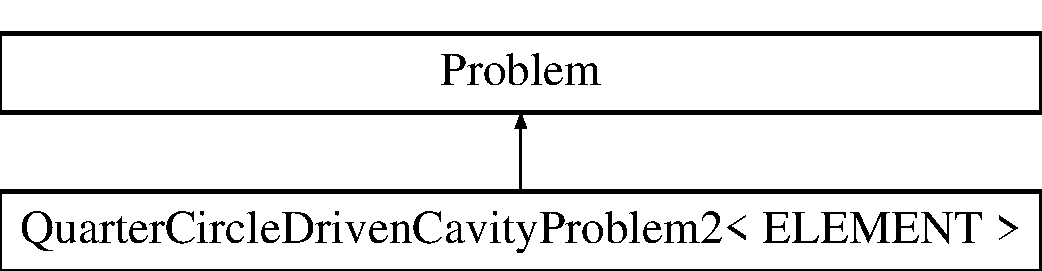
\includegraphics[height=2.000000cm]{classQuarterCircleDrivenCavityProblem2}
\end{center}
\end{figure}
\subsection*{Public Member Functions}
\begin{DoxyCompactItemize}
\item 
\hyperlink{classQuarterCircleDrivenCavityProblem2_a301f6d2c50e2d266126a80956397d78d}{Quarter\+Circle\+Driven\+Cavity\+Problem2} (Navier\+Stokes\+Equations$<$ 2 $>$\+::Navier\+Stokes\+Body\+Force\+Fct\+Pt body\+\_\+force\+\_\+fct\+\_\+pt)
\begin{DoxyCompactList}\small\item\em Constructor. \end{DoxyCompactList}\item 
\hyperlink{classQuarterCircleDrivenCavityProblem2_afaedf67201056ed5466b139d2bb58d61}{$\sim$\+Quarter\+Circle\+Driven\+Cavity\+Problem2} ()
\begin{DoxyCompactList}\small\item\em Destructor\+: Empty. \end{DoxyCompactList}\item 
void \hyperlink{classQuarterCircleDrivenCavityProblem2_a1417ca3cc4a838d407c8bf85372dfc8f}{actions\+\_\+after\+\_\+newton\+\_\+solve} ()
\begin{DoxyCompactList}\small\item\em Update the after solve (empty) \end{DoxyCompactList}\item 
void \hyperlink{classQuarterCircleDrivenCavityProblem2_aed64247640938ca570da33238e9696ac}{actions\+\_\+before\+\_\+newton\+\_\+solve} ()
\begin{DoxyCompactList}\small\item\em Update the problem specs before solve. (Re-\/)set velocity boundary conditions just to be on the safe side... \end{DoxyCompactList}\item 
void \hyperlink{classQuarterCircleDrivenCavityProblem2_a51d108d18f50d81bad0da998741254a9}{actions\+\_\+after\+\_\+adapt} ()
\begin{DoxyCompactList}\small\item\em After adaptation\+: Unpin pressure and pin redudant pressure dofs. \end{DoxyCompactList}\item 
void \hyperlink{classQuarterCircleDrivenCavityProblem2_a506c1a77cc9a11f586f5cc1b4a252798}{doc\+\_\+solution} (Doc\+Info \&doc\+\_\+info)
\begin{DoxyCompactList}\small\item\em Doc the solution. \end{DoxyCompactList}\end{DoxyCompactItemize}
\subsection*{Private Member Functions}
\begin{DoxyCompactItemize}
\item 
void \hyperlink{classQuarterCircleDrivenCavityProblem2_ae5ce524af511e8399cd5f261afe9331f}{fix\+\_\+pressure} (const unsigned \&e, const unsigned \&pdof, const double \&pvalue)
\begin{DoxyCompactList}\small\item\em Fix pressure in element e at pressure dof pdof and set to pvalue. \end{DoxyCompactList}\end{DoxyCompactItemize}
\subsection*{Private Attributes}
\begin{DoxyCompactItemize}
\item 
Navier\+Stokes\+Equations$<$ 2 $>$\+::Navier\+Stokes\+Body\+Force\+Fct\+Pt \hyperlink{classQuarterCircleDrivenCavityProblem2_ad2b3c4fdc4136aebc331f44cbe13421b}{Body\+\_\+force\+\_\+fct\+\_\+pt}
\begin{DoxyCompactList}\small\item\em Pointer to body force function. \end{DoxyCompactList}\end{DoxyCompactItemize}


\subsection{Detailed Description}
\subsubsection*{template$<$class E\+L\+E\+M\+E\+NT$>$\newline
class Quarter\+Circle\+Driven\+Cavity\+Problem2$<$ E\+L\+E\+M\+E\+N\+T $>$}

Driven cavity problem in quarter circle domain, templated by element type. 

Definition at line 88 of file circular\+\_\+driven\+\_\+cavity2.\+cc.



\subsection{Constructor \& Destructor Documentation}
\mbox{\Hypertarget{classQuarterCircleDrivenCavityProblem2_a301f6d2c50e2d266126a80956397d78d}\label{classQuarterCircleDrivenCavityProblem2_a301f6d2c50e2d266126a80956397d78d}} 
\index{Quarter\+Circle\+Driven\+Cavity\+Problem2@{Quarter\+Circle\+Driven\+Cavity\+Problem2}!Quarter\+Circle\+Driven\+Cavity\+Problem2@{Quarter\+Circle\+Driven\+Cavity\+Problem2}}
\index{Quarter\+Circle\+Driven\+Cavity\+Problem2@{Quarter\+Circle\+Driven\+Cavity\+Problem2}!Quarter\+Circle\+Driven\+Cavity\+Problem2@{Quarter\+Circle\+Driven\+Cavity\+Problem2}}
\subsubsection{\texorpdfstring{Quarter\+Circle\+Driven\+Cavity\+Problem2()}{QuarterCircleDrivenCavityProblem2()}}
{\footnotesize\ttfamily template$<$class E\+L\+E\+M\+E\+NT $>$ \\
\hyperlink{classQuarterCircleDrivenCavityProblem2}{Quarter\+Circle\+Driven\+Cavity\+Problem2}$<$ E\+L\+E\+M\+E\+NT $>$\+::\hyperlink{classQuarterCircleDrivenCavityProblem2}{Quarter\+Circle\+Driven\+Cavity\+Problem2} (\begin{DoxyParamCaption}\item[{Navier\+Stokes\+Equations$<$ 2 $>$\+::Navier\+Stokes\+Body\+Force\+Fct\+Pt}]{body\+\_\+force\+\_\+fct\+\_\+pt }\end{DoxyParamCaption})}



Constructor. 

Constructor for driven cavity problem in quarter circle domain. 

Definition at line 189 of file circular\+\_\+driven\+\_\+cavity2.\+cc.



References Quarter\+Circle\+Driven\+Cavity\+Problem2$<$ E\+L\+E\+M\+E\+N\+T $>$\+::\+Body\+\_\+force\+\_\+fct\+\_\+pt, Quarter\+Circle\+Driven\+Cavity\+Problem2$<$ E\+L\+E\+M\+E\+N\+T $>$\+::fix\+\_\+pressure(), Global\+\_\+\+Physical\+\_\+\+Variables2\+::\+Gravity(), Global\+\_\+\+Physical\+\_\+\+Variables2\+::\+Re, and Global\+\_\+\+Physical\+\_\+\+Variables2\+::\+Re\+\_\+inv\+Fr.

\mbox{\Hypertarget{classQuarterCircleDrivenCavityProblem2_afaedf67201056ed5466b139d2bb58d61}\label{classQuarterCircleDrivenCavityProblem2_afaedf67201056ed5466b139d2bb58d61}} 
\index{Quarter\+Circle\+Driven\+Cavity\+Problem2@{Quarter\+Circle\+Driven\+Cavity\+Problem2}!````~Quarter\+Circle\+Driven\+Cavity\+Problem2@{$\sim$\+Quarter\+Circle\+Driven\+Cavity\+Problem2}}
\index{````~Quarter\+Circle\+Driven\+Cavity\+Problem2@{$\sim$\+Quarter\+Circle\+Driven\+Cavity\+Problem2}!Quarter\+Circle\+Driven\+Cavity\+Problem2@{Quarter\+Circle\+Driven\+Cavity\+Problem2}}
\subsubsection{\texorpdfstring{$\sim$\+Quarter\+Circle\+Driven\+Cavity\+Problem2()}{~QuarterCircleDrivenCavityProblem2()}}
{\footnotesize\ttfamily template$<$class E\+L\+E\+M\+E\+NT$>$ \\
\hyperlink{classQuarterCircleDrivenCavityProblem2}{Quarter\+Circle\+Driven\+Cavity\+Problem2}$<$ E\+L\+E\+M\+E\+NT $>$\+::$\sim$\hyperlink{classQuarterCircleDrivenCavityProblem2}{Quarter\+Circle\+Driven\+Cavity\+Problem2} (\begin{DoxyParamCaption}{ }\end{DoxyParamCaption})\hspace{0.3cm}{\ttfamily [inline]}}



Destructor\+: Empty. 



Definition at line 98 of file circular\+\_\+driven\+\_\+cavity2.\+cc.



\subsection{Member Function Documentation}
\mbox{\Hypertarget{classQuarterCircleDrivenCavityProblem2_a51d108d18f50d81bad0da998741254a9}\label{classQuarterCircleDrivenCavityProblem2_a51d108d18f50d81bad0da998741254a9}} 
\index{Quarter\+Circle\+Driven\+Cavity\+Problem2@{Quarter\+Circle\+Driven\+Cavity\+Problem2}!actions\+\_\+after\+\_\+adapt@{actions\+\_\+after\+\_\+adapt}}
\index{actions\+\_\+after\+\_\+adapt@{actions\+\_\+after\+\_\+adapt}!Quarter\+Circle\+Driven\+Cavity\+Problem2@{Quarter\+Circle\+Driven\+Cavity\+Problem2}}
\subsubsection{\texorpdfstring{actions\+\_\+after\+\_\+adapt()}{actions\_after\_adapt()}}
{\footnotesize\ttfamily template$<$class E\+L\+E\+M\+E\+NT$>$ \\
void \hyperlink{classQuarterCircleDrivenCavityProblem2}{Quarter\+Circle\+Driven\+Cavity\+Problem2}$<$ E\+L\+E\+M\+E\+NT $>$\+::actions\+\_\+after\+\_\+adapt (\begin{DoxyParamCaption}{ }\end{DoxyParamCaption})\hspace{0.3cm}{\ttfamily [inline]}}



After adaptation\+: Unpin pressure and pin redudant pressure dofs. 



Definition at line 150 of file circular\+\_\+driven\+\_\+cavity2.\+cc.

\mbox{\Hypertarget{classQuarterCircleDrivenCavityProblem2_a1417ca3cc4a838d407c8bf85372dfc8f}\label{classQuarterCircleDrivenCavityProblem2_a1417ca3cc4a838d407c8bf85372dfc8f}} 
\index{Quarter\+Circle\+Driven\+Cavity\+Problem2@{Quarter\+Circle\+Driven\+Cavity\+Problem2}!actions\+\_\+after\+\_\+newton\+\_\+solve@{actions\+\_\+after\+\_\+newton\+\_\+solve}}
\index{actions\+\_\+after\+\_\+newton\+\_\+solve@{actions\+\_\+after\+\_\+newton\+\_\+solve}!Quarter\+Circle\+Driven\+Cavity\+Problem2@{Quarter\+Circle\+Driven\+Cavity\+Problem2}}
\subsubsection{\texorpdfstring{actions\+\_\+after\+\_\+newton\+\_\+solve()}{actions\_after\_newton\_solve()}}
{\footnotesize\ttfamily template$<$class E\+L\+E\+M\+E\+NT$>$ \\
void \hyperlink{classQuarterCircleDrivenCavityProblem2}{Quarter\+Circle\+Driven\+Cavity\+Problem2}$<$ E\+L\+E\+M\+E\+NT $>$\+::actions\+\_\+after\+\_\+newton\+\_\+solve (\begin{DoxyParamCaption}{ }\end{DoxyParamCaption})\hspace{0.3cm}{\ttfamily [inline]}}



Update the after solve (empty) 



Definition at line 101 of file circular\+\_\+driven\+\_\+cavity2.\+cc.

\mbox{\Hypertarget{classQuarterCircleDrivenCavityProblem2_aed64247640938ca570da33238e9696ac}\label{classQuarterCircleDrivenCavityProblem2_aed64247640938ca570da33238e9696ac}} 
\index{Quarter\+Circle\+Driven\+Cavity\+Problem2@{Quarter\+Circle\+Driven\+Cavity\+Problem2}!actions\+\_\+before\+\_\+newton\+\_\+solve@{actions\+\_\+before\+\_\+newton\+\_\+solve}}
\index{actions\+\_\+before\+\_\+newton\+\_\+solve@{actions\+\_\+before\+\_\+newton\+\_\+solve}!Quarter\+Circle\+Driven\+Cavity\+Problem2@{Quarter\+Circle\+Driven\+Cavity\+Problem2}}
\subsubsection{\texorpdfstring{actions\+\_\+before\+\_\+newton\+\_\+solve()}{actions\_before\_newton\_solve()}}
{\footnotesize\ttfamily template$<$class E\+L\+E\+M\+E\+NT$>$ \\
void \hyperlink{classQuarterCircleDrivenCavityProblem2}{Quarter\+Circle\+Driven\+Cavity\+Problem2}$<$ E\+L\+E\+M\+E\+NT $>$\+::actions\+\_\+before\+\_\+newton\+\_\+solve (\begin{DoxyParamCaption}{ }\end{DoxyParamCaption})\hspace{0.3cm}{\ttfamily [inline]}}



Update the problem specs before solve. (Re-\/)set velocity boundary conditions just to be on the safe side... 



Definition at line 105 of file circular\+\_\+driven\+\_\+cavity2.\+cc.

\mbox{\Hypertarget{classQuarterCircleDrivenCavityProblem2_a506c1a77cc9a11f586f5cc1b4a252798}\label{classQuarterCircleDrivenCavityProblem2_a506c1a77cc9a11f586f5cc1b4a252798}} 
\index{Quarter\+Circle\+Driven\+Cavity\+Problem2@{Quarter\+Circle\+Driven\+Cavity\+Problem2}!doc\+\_\+solution@{doc\+\_\+solution}}
\index{doc\+\_\+solution@{doc\+\_\+solution}!Quarter\+Circle\+Driven\+Cavity\+Problem2@{Quarter\+Circle\+Driven\+Cavity\+Problem2}}
\subsubsection{\texorpdfstring{doc\+\_\+solution()}{doc\_solution()}}
{\footnotesize\ttfamily template$<$class E\+L\+E\+M\+E\+NT $>$ \\
void \hyperlink{classQuarterCircleDrivenCavityProblem2}{Quarter\+Circle\+Driven\+Cavity\+Problem2}$<$ E\+L\+E\+M\+E\+NT $>$\+::doc\+\_\+solution (\begin{DoxyParamCaption}\item[{Doc\+Info \&}]{doc\+\_\+info }\end{DoxyParamCaption})}



Doc the solution. 



Definition at line 280 of file circular\+\_\+driven\+\_\+cavity2.\+cc.



Referenced by main().

\mbox{\Hypertarget{classQuarterCircleDrivenCavityProblem2_ae5ce524af511e8399cd5f261afe9331f}\label{classQuarterCircleDrivenCavityProblem2_ae5ce524af511e8399cd5f261afe9331f}} 
\index{Quarter\+Circle\+Driven\+Cavity\+Problem2@{Quarter\+Circle\+Driven\+Cavity\+Problem2}!fix\+\_\+pressure@{fix\+\_\+pressure}}
\index{fix\+\_\+pressure@{fix\+\_\+pressure}!Quarter\+Circle\+Driven\+Cavity\+Problem2@{Quarter\+Circle\+Driven\+Cavity\+Problem2}}
\subsubsection{\texorpdfstring{fix\+\_\+pressure()}{fix\_pressure()}}
{\footnotesize\ttfamily template$<$class E\+L\+E\+M\+E\+NT$>$ \\
void \hyperlink{classQuarterCircleDrivenCavityProblem2}{Quarter\+Circle\+Driven\+Cavity\+Problem2}$<$ E\+L\+E\+M\+E\+NT $>$\+::fix\+\_\+pressure (\begin{DoxyParamCaption}\item[{const unsigned \&}]{e,  }\item[{const unsigned \&}]{pdof,  }\item[{const double \&}]{pvalue }\end{DoxyParamCaption})\hspace{0.3cm}{\ttfamily [inline]}, {\ttfamily [private]}}



Fix pressure in element e at pressure dof pdof and set to pvalue. 



Definition at line 173 of file circular\+\_\+driven\+\_\+cavity2.\+cc.



Referenced by Quarter\+Circle\+Driven\+Cavity\+Problem2$<$ E\+L\+E\+M\+E\+N\+T $>$\+::\+Quarter\+Circle\+Driven\+Cavity\+Problem2().



\subsection{Member Data Documentation}
\mbox{\Hypertarget{classQuarterCircleDrivenCavityProblem2_ad2b3c4fdc4136aebc331f44cbe13421b}\label{classQuarterCircleDrivenCavityProblem2_ad2b3c4fdc4136aebc331f44cbe13421b}} 
\index{Quarter\+Circle\+Driven\+Cavity\+Problem2@{Quarter\+Circle\+Driven\+Cavity\+Problem2}!Body\+\_\+force\+\_\+fct\+\_\+pt@{Body\+\_\+force\+\_\+fct\+\_\+pt}}
\index{Body\+\_\+force\+\_\+fct\+\_\+pt@{Body\+\_\+force\+\_\+fct\+\_\+pt}!Quarter\+Circle\+Driven\+Cavity\+Problem2@{Quarter\+Circle\+Driven\+Cavity\+Problem2}}
\subsubsection{\texorpdfstring{Body\+\_\+force\+\_\+fct\+\_\+pt}{Body\_force\_fct\_pt}}
{\footnotesize\ttfamily template$<$class E\+L\+E\+M\+E\+NT$>$ \\
Navier\+Stokes\+Equations$<$2$>$\+::Navier\+Stokes\+Body\+Force\+Fct\+Pt \hyperlink{classQuarterCircleDrivenCavityProblem2}{Quarter\+Circle\+Driven\+Cavity\+Problem2}$<$ E\+L\+E\+M\+E\+NT $>$\+::Body\+\_\+force\+\_\+fct\+\_\+pt\hspace{0.3cm}{\ttfamily [private]}}



Pointer to body force function. 



Definition at line 170 of file circular\+\_\+driven\+\_\+cavity2.\+cc.



Referenced by Quarter\+Circle\+Driven\+Cavity\+Problem2$<$ E\+L\+E\+M\+E\+N\+T $>$\+::\+Quarter\+Circle\+Driven\+Cavity\+Problem2().



The documentation for this class was generated from the following file\+:\begin{DoxyCompactItemize}
\item 
\hyperlink{circular__driven__cavity2_8cc}{circular\+\_\+driven\+\_\+cavity2.\+cc}\end{DoxyCompactItemize}

\chapter{File Documentation}
\hypertarget{circular__driven__cavity_8cc}{}\section{circular\+\_\+driven\+\_\+cavity.\+cc File Reference}
\label{circular__driven__cavity_8cc}\index{circular\+\_\+driven\+\_\+cavity.\+cc@{circular\+\_\+driven\+\_\+cavity.\+cc}}
\subsection*{Classes}
\begin{DoxyCompactItemize}
\item 
class \hyperlink{classQuarterCircleDrivenCavityProblem}{Quarter\+Circle\+Driven\+Cavity\+Problem$<$ E\+L\+E\+M\+E\+N\+T $>$}
\end{DoxyCompactItemize}
\subsection*{Namespaces}
\begin{DoxyCompactItemize}
\item 
 \hyperlink{namespaceGlobal__Physical__Variables}{Global\+\_\+\+Physical\+\_\+\+Variables}
\begin{DoxyCompactList}\small\item\em Namespace for physical parameters. \end{DoxyCompactList}\end{DoxyCompactItemize}
\subsection*{Functions}
\begin{DoxyCompactItemize}
\item 
Vector$<$ double $>$ \hyperlink{namespaceGlobal__Physical__Variables_afae321364975eb56688ad13abc8ed6b7}{Global\+\_\+\+Physical\+\_\+\+Variables\+::\+Gravity} (2)
\begin{DoxyCompactList}\small\item\em Gravity vector. \end{DoxyCompactList}\item 
void \hyperlink{namespaceGlobal__Physical__Variables_a87da705b8a46bed337cf5dbdd788b87b}{Global\+\_\+\+Physical\+\_\+\+Variables\+::body\+\_\+force} (const double \&time, const Vector$<$ double $>$ \&x, Vector$<$ double $>$ \&result)
\begin{DoxyCompactList}\small\item\em Functional body force. \end{DoxyCompactList}\item 
void \hyperlink{namespaceGlobal__Physical__Variables_a9780d615ae07c4e00a436ab2973b54e6}{Global\+\_\+\+Physical\+\_\+\+Variables\+::zero\+\_\+body\+\_\+force} (const double \&time, const Vector$<$ double $>$ \&x, Vector$<$ double $>$ \&result)
\begin{DoxyCompactList}\small\item\em Zero functional body force. \end{DoxyCompactList}\item 
int \hyperlink{circular__driven__cavity_8cc_ae66f6b31b5ad750f1fe042a706a4e3d4}{main} ()
\begin{DoxyCompactList}\small\item\em Driver for \hyperlink{classQuarterCircleDrivenCavityProblem}{Quarter\+Circle\+Driven\+Cavity\+Problem} test problem. \end{DoxyCompactList}\end{DoxyCompactItemize}
\subsection*{Variables}
\begin{DoxyCompactItemize}
\item 
double \hyperlink{namespaceGlobal__Physical__Variables_ab814e627d2eb5bc50318879d19ab16b9}{Global\+\_\+\+Physical\+\_\+\+Variables\+::\+Re} =100
\begin{DoxyCompactList}\small\item\em Reynolds number. \end{DoxyCompactList}\item 
double \hyperlink{namespaceGlobal__Physical__Variables_ab1a845a672b4d74b304639a976dc65c6}{Global\+\_\+\+Physical\+\_\+\+Variables\+::\+Re\+\_\+inv\+Fr} =100
\begin{DoxyCompactList}\small\item\em Reynolds/\+Froude number. \end{DoxyCompactList}\end{DoxyCompactItemize}


\subsection{Function Documentation}
\mbox{\Hypertarget{circular__driven__cavity_8cc_ae66f6b31b5ad750f1fe042a706a4e3d4}\label{circular__driven__cavity_8cc_ae66f6b31b5ad750f1fe042a706a4e3d4}} 
\index{circular\+\_\+driven\+\_\+cavity.\+cc@{circular\+\_\+driven\+\_\+cavity.\+cc}!main@{main}}
\index{main@{main}!circular\+\_\+driven\+\_\+cavity.\+cc@{circular\+\_\+driven\+\_\+cavity.\+cc}}
\subsubsection{\texorpdfstring{main()}{main()}}
{\footnotesize\ttfamily int main (\begin{DoxyParamCaption}{ }\end{DoxyParamCaption})}



Driver for \hyperlink{classQuarterCircleDrivenCavityProblem}{Quarter\+Circle\+Driven\+Cavity\+Problem} test problem. 



Definition at line 292 of file circular\+\_\+driven\+\_\+cavity.\+cc.



References Global\+\_\+\+Physical\+\_\+\+Variables\+::body\+\_\+force(), Quarter\+Circle\+Driven\+Cavity\+Problem$<$ E\+L\+E\+M\+E\+N\+T $>$\+::doc\+\_\+solution(), Global\+\_\+\+Physical\+\_\+\+Variables\+::\+Gravity(), and Global\+\_\+\+Physical\+\_\+\+Variables\+::zero\+\_\+body\+\_\+force().


\hypertarget{circular__driven__cavity_8txt__doxygenified_8h}{}\section{circular\+\_\+driven\+\_\+cavity.\+txt\+\_\+doxygenified.\+h File Reference}
\label{circular__driven__cavity_8txt__doxygenified_8h}\index{circular\+\_\+driven\+\_\+cavity.\+txt\+\_\+doxygenified.\+h@{circular\+\_\+driven\+\_\+cavity.\+txt\+\_\+doxygenified.\+h}}

\hypertarget{circular__driven__cavity2_8cc}{}\section{circular\+\_\+driven\+\_\+cavity2.\+cc File Reference}
\label{circular__driven__cavity2_8cc}\index{circular\+\_\+driven\+\_\+cavity2.\+cc@{circular\+\_\+driven\+\_\+cavity2.\+cc}}
\subsection*{Classes}
\begin{DoxyCompactItemize}
\item 
class \hyperlink{classQuarterCircleDrivenCavityProblem2}{Quarter\+Circle\+Driven\+Cavity\+Problem2$<$ E\+L\+E\+M\+E\+N\+T $>$}
\end{DoxyCompactItemize}
\subsection*{Namespaces}
\begin{DoxyCompactItemize}
\item 
 \hyperlink{namespaceGlobal__Physical__Variables2}{Global\+\_\+\+Physical\+\_\+\+Variables2}
\begin{DoxyCompactList}\small\item\em Namespace for physical parameters. \end{DoxyCompactList}\end{DoxyCompactItemize}
\subsection*{Functions}
\begin{DoxyCompactItemize}
\item 
Vector$<$ double $>$ \hyperlink{namespaceGlobal__Physical__Variables2_a302cf0e32c91f4d73a96cca3db4525bb}{Global\+\_\+\+Physical\+\_\+\+Variables2\+::\+Gravity} (2)
\begin{DoxyCompactList}\small\item\em Gravity vector. \end{DoxyCompactList}\item 
void \hyperlink{namespaceGlobal__Physical__Variables2_a81f723c56b35c14482cc516f0bfce3cd}{Global\+\_\+\+Physical\+\_\+\+Variables2\+::body\+\_\+force} (const double \&time, const Vector$<$ double $>$ \&x, Vector$<$ double $>$ \&result)
\begin{DoxyCompactList}\small\item\em Functional body force. \end{DoxyCompactList}\item 
void \hyperlink{namespaceGlobal__Physical__Variables2_a3820ea1a672c3e2709095fc366e40ca7}{Global\+\_\+\+Physical\+\_\+\+Variables2\+::zero\+\_\+body\+\_\+force} (const double \&time, const Vector$<$ double $>$ \&x, Vector$<$ double $>$ \&result)
\begin{DoxyCompactList}\small\item\em Zero functional body force. \end{DoxyCompactList}\item 
int \hyperlink{circular__driven__cavity2_8cc_ae66f6b31b5ad750f1fe042a706a4e3d4}{main} ()
\begin{DoxyCompactList}\small\item\em Driver for \hyperlink{classQuarterCircleDrivenCavityProblem2}{Quarter\+Circle\+Driven\+Cavity\+Problem2} test problem. \end{DoxyCompactList}\end{DoxyCompactItemize}
\subsection*{Variables}
\begin{DoxyCompactItemize}
\item 
double \hyperlink{namespaceGlobal__Physical__Variables2_afce617c1bd6726b29fa0e1f7c892a955}{Global\+\_\+\+Physical\+\_\+\+Variables2\+::\+Re} =100
\begin{DoxyCompactList}\small\item\em Reynolds number. \end{DoxyCompactList}\item 
double \hyperlink{namespaceGlobal__Physical__Variables2_a29c665c13064cdd6ecbb6c6ab654f743}{Global\+\_\+\+Physical\+\_\+\+Variables2\+::\+Re\+\_\+inv\+Fr} =100
\begin{DoxyCompactList}\small\item\em Reynolds/\+Froude number. \end{DoxyCompactList}\end{DoxyCompactItemize}


\subsection{Function Documentation}
\mbox{\Hypertarget{circular__driven__cavity2_8cc_ae66f6b31b5ad750f1fe042a706a4e3d4}\label{circular__driven__cavity2_8cc_ae66f6b31b5ad750f1fe042a706a4e3d4}} 
\index{circular\+\_\+driven\+\_\+cavity2.\+cc@{circular\+\_\+driven\+\_\+cavity2.\+cc}!main@{main}}
\index{main@{main}!circular\+\_\+driven\+\_\+cavity2.\+cc@{circular\+\_\+driven\+\_\+cavity2.\+cc}}
\subsubsection{\texorpdfstring{main()}{main()}}
{\footnotesize\ttfamily int main (\begin{DoxyParamCaption}{ }\end{DoxyParamCaption})}



Driver for \hyperlink{classQuarterCircleDrivenCavityProblem2}{Quarter\+Circle\+Driven\+Cavity\+Problem2} test problem. 



Definition at line 305 of file circular\+\_\+driven\+\_\+cavity2.\+cc.



References Global\+\_\+\+Physical\+\_\+\+Variables2\+::body\+\_\+force(), Quarter\+Circle\+Driven\+Cavity\+Problem2$<$ E\+L\+E\+M\+E\+N\+T $>$\+::doc\+\_\+solution(), Global\+\_\+\+Physical\+\_\+\+Variables2\+::\+Gravity(), and Global\+\_\+\+Physical\+\_\+\+Variables2\+::zero\+\_\+body\+\_\+force().


%--- End generated contents ---

% Index
\backmatter
\newpage
\phantomsection
\clearemptydoublepage
\addcontentsline{toc}{chapter}{Index}
\printindex

